\documentclass[12pt,letter]{article}
\usepackage{graphicx}


\title{Homework Two Report}
\author{University of Victoria\\Instructor: Xuekui Zhang\\Zhaocheng Li (V00832770)}
\begin{document}
\maketitle
\begin{abstract}
	The report demostrates the prediction performance without stacking procedure. Thus the goal is very similar to frist assignment's goal. But differently, we apply classification method (cutoff) this time.
	
	In order to assess the performance of each model, we construct the miss classification table and calculate the miss classification rate. Be aware that the lower the rate is, the better the model prediction gets.
	
	Notice that although this assignment is much simplified, it takes significant runtime. I separate the $glmnet()$ functions from the rest.
\end{abstract}
\section{Instruciton}
Please following the $README$ file, which explains in detail how my program works.\\
\vspace{1mm}\\
Basically, for grading process, the tutor does not have to make any modification except, the working directory. Whoever running the program should adjust the working directory accordingly. \\
\vspace{1mm}\\
The working directory is listed at the top of code.

\section{Code Skeleton}
This section I will brief the basic skeleton of my entire code file to ease the workload of the grader, given the massive data needed to process.
\subsection{dataset loading}
In the first, of course, we are going to load the data into program and modify them into desirable format. To achieve this goal, we here apply the professor's $Helperfunctions.R$ to do so.\\
\vspace{1mm}\\
In the end of this part, we will have a matrix that contains the outcomes of five drugs (continuous response) and corresponding mutual gene status (discrete variables). We also have the our needed libraries ready to use later.

\subsection{function preparation}
I have created three main strucutures I need to use throughout the code. The $cutoff$ function is used in classification process, making a matrix of continuous y-values (5 drugs outcomes) as input and transform it into a matrix of discrete values (0's and 1's);\\
\vspace{1mm}\\
Also, the $reorder$ function is used in converting unorder matrix into one by the order of $columnnames$.\\
\vspace{1mm}\\
At the end, there is a 8-by-20 matrix defined at first, called $Matrix$, which is a storage to save the miss classification rates for eight models, in 20 seeds (a ramdom index). This is basically the result we want to have and study for this assignment.\\
\vspace{1mm}\\
In addtion, there are also alot minor temporary data structures I use in the middle of computation, and I will demonstrate their uses in comments as I use them.

\subsection{method one \& analyzing first four models}
I did not include set of $glmnet$ functions here, but separate them into the following individual section. This is due to the consideration of massive runtime for running all of them together. Although the fact suggests that in the way, it still costs significantly long runtime.\\
\vspace{1mm}\\
As required, in this part, before comparing the methods in 20 loops with 5-fold cross validation, we need to go through the $cutoff$ with matrix first, to make it a $discrete-valued$ matrix. This is method one. And the models we assess are logistic regression, LDA, KNN, and classification tree.

\subsection{method two \& analyzing another two models}
Similarly, we leave out the family of $glmnet$ functions. The models we uses here are linear regression and regression tree.\\
\vspace{1mm}\\
Method two simply means that we predict first using the continuous variables, then convert them into discrete variable using $cutoff$ function.

\subsection{method 1,2 \& analyzing penalized regression}
Then we will study the glmnet functions here using the two methods, repectively.\\
\vspace{1mm}\\
Notice that this is a huge workload computationally because there are 11 models to process each time, including Lasso, Ridge, and other elastic net functions. And in comparison we pick the one with best peroformance, i.e. the one with lowest miss classification rate, to take into consideration.

\section{Outcome Display}
The table $Matrix$ shown below is recording the miss classification rate for each model in each random seed out of 20. It represents how the model behaves and it gives us better chance to know more by analyzing on it.\\
\vspace{1mm}\\
Of course, we can easily see, for each model, different distribution of sets in cross-validation (the change of seeds) does not incluence its behaviour. Each model performs steadily among all seeds. Which will ensure a convincing outcome of analysis.

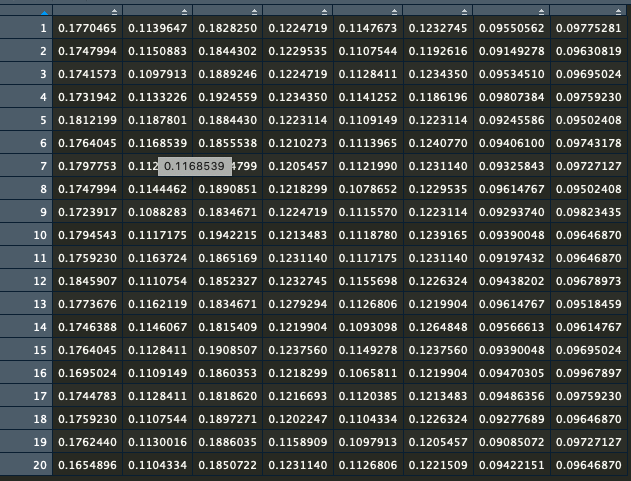
\includegraphics[scale=0.5]{Matrix.png}\\
This is the type of solution matrix we can get, 8 models, 20 seeds, miss classification rate in each table 

\section{Findings}
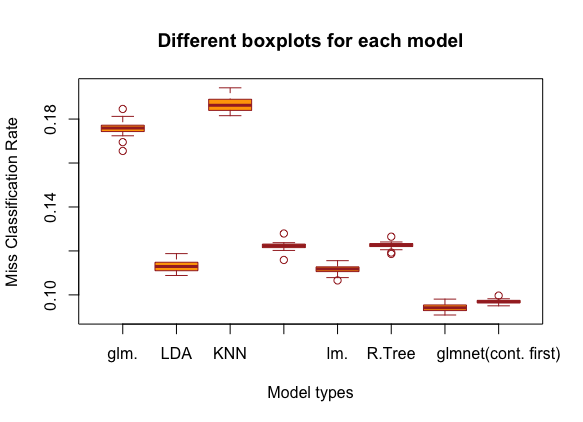
\includegraphics[scale=0.5]{Rplot.png}\\
By the solution matrix, we have constructed a system of boxplots for each model, we can see that the highest miss classification rate is KNN, and maybe glm as well. And it may indicates a relative poor performance of prediction.\\
However, the glmnet functions are the most accurate function to make prediction, and the glmnet using cutoff first is lowest. It performs very well.

\end{document}
